\documentclass[]{article}

\usepackage{amsmath}
\usepackage{graphicx}
\graphicspath{ {./figures/} }

%opening
\title{Magical ecologies: a model of predator-prey equilibria for closed systems of magical girls and witches}
\author{Kyubey \#65471}

\begin{document}

\maketitle

\begin{abstract}
	We present a simple mathematical model of interactions between magical girl (\textit{Puella Magica}) and witch (\textit{Maga Malefica}) populations in a closed regulated system. The model makes use of a few descriptive parameters to characterise the environment and predicts dynamical population behaviour. We show how some very general conclusions can be deduced about the equilibrium populations of magical girls and witches and their stability. This study will provide operators in the field with more tools to better manage the ecology of these species, which are vital for our universe's thermodynamic preservation. 
\end{abstract}

\section{Introduction}

Since the first documented discovery of the exothermic, anentropic decay process from magical girl (\textit{Puella Magica}) to witch (\textit{Maga Malefica}) \cite{kyubey1}, this fundamental phenomenon has become a key element of our species' activities in the field of cosmic scale thermodynamic preservation. The management of magical girl-witch ecologies has today a disproportionate impact on our economy, employing effectively 99.93\% of our active population, and providing a free energy flux of more than $10^{40} W$ across all the galaxies over which we've currently spread. While this is still far below the amount necessary to definitely stave off heat death, the impressive scale and efficiency of this operation can not be overstated. It is thus somewhat surprising that until now the management of local ecologies has often been left to individual operators, almost as an art more than a science. While this has often been successful, occasional examples of ecological collapses on a catastrophic scale have been recorded \cite{kyubey2}. Therefore, we endeavour here to begin an attempt at a systematic description of magical girl-witch ecological equilibria, as a tool for future control and regulation of such system.

\section{The model}

Let us consider a closed system containing two populations of magical girls and witches, labelled respectively as $M$ and $W$. The indigenous species is here considered as a virtually infinite reserve; this is in general a good approximation, and we will see later that it is not a problem for the results of the model. We then consider the dynamics affecting these populations. For magical girls, three phenomena are at play:

\begin{enumerate}
	\item a recruitment process by the local Kyubey agent;
	\item a loss to witches in battle;
	\item a loss to decay processes and transformation into witches.
\end{enumerate}

Conversely, for witches, there are only two relevant phenomena:

\begin{enumerate}
	\item an increase in numbers thanks to decay processes of magical girls;
	\item a loss to magical girls in battle.
\end{enumerate}

In order to fully characterise this system we introduce five parameters. The first is the recruitment rate, $r$. The second is the probability of battle $b$; this is chosen so that the total number of battles per unit time can be found as $N_B = bMW$. Since $MW$ is proportional to the likelihood of a clash between magical girls and witches, which increases with both their population, $b$ depends in general by the area over which these population are spread. For a large city, for example, $b$ will be small, as encounters are less likely unless the populations are large enough to compensate. Other local factors however can affect $b$, such as the attitudes and motivation level of the local population of magical girls and the general psychological state of the indigenous community, which has an effect on witch activity.\newline
The third parameter is the win rate, $w$ (not to be confused with the witch population, $W$). This expresses simply the likelihood of the average magical girl defeating the average witch in battle, so it has to be $0 \leq w \leq 1$. The last two parameters are inherent to the qualities of the soul gems of the local magical girls. These are the average decay time, $\tau_0$, which represents the average time a magical girl would decay into a witch if deprived of any means to recharge her soul gem, and the efficiency of recharge, $\eta$, which represents the average fraction of a soul gem's total energy that can be recovered with a grief seed. While it has to be $\eta \geq 0$, there is no upper limit; soul gems can not be overcharged, but nothing forbids magical girls from saving partially used-up grief seeds to use for future recharges if they manage to do so. However, in practice, it tends to be that $\eta \sim 0.25$.\newline

We can now outline the dynamical equations of the model. These are a pair of first order differential equations:

\begin{equation}\label{eq_mg}
\frac{dM}{dt} = r-\frac{1}{\tau_0+\eta b w W}M-b (1-w)MW 
\end{equation}

\begin{equation}\label{eq_w}
\frac{dW}{dt} = \frac{1}{\tau_0+\eta b w W}M-bwMW 
\end{equation}

Most of these terms are self-explanatory. The magical girls creation rate $r$ is the only positive contribution to $dM/dt$, and losses to battles are represented as $N_B$ multiplied by the likelihood of unfavourable outcome for each party, respectively, $1-w$ and $w$ for magical girls and witches. However, the decay process deserves a bit more of attention. We have here made use of an effective decay rate,

\begin{equation}\label{tau}
\tau = \tau_0+\frac{\eta w N_B}{M} = \tau_0+\eta b w W
\end{equation}

. In other words, we consider an extension to the regular decay time that is proportional to how many witches each magical girls gets to defeat, on average, times the efficiency $\eta$.\newline
We now move on to study this model in some detail. As we will see, it leads to surprising and useful insights about the equilibria of magical girls and witches, and the resulting energy production.

\section{Results}
\subsection{Equilibrium}

To search for the equilibrium conditions of this model we look for values of $M$ and $W$ which cause Eq. \ref{eq_mg} and \ref{eq_w} to be zero. This turns out to be actually quite simple. If we focus on \ref{eq_w}, we see that since $M$ appears in both terms, it can be simplified. This leads us to the first important finding of this work: \textit{the equilibrium population of witches is independent from the amount of magical girls present}. In particular, by solving a second degree equation and discarding the unphysical negative solution, we find

\begin{equation}\label{eq_pop_w}
W_{eq} = \frac{\sqrt{\tau_0^2+4\eta}-\tau_0}{2\eta bw}
\end{equation}

. In other words, the equilibrium population for witches only depends on the average properties of soul gems and on other local factors such as the area of the habitat in which they're living and the combat skill of the magical girls. In particulars, since it's reasonable to assume that $b \sim 1/A$, where $A$ is the area of the habitat, this leads to a constant sustainable density of witches that only depends on the properties of the local population of magical girls and indigenous species.\newline
Having found this equilibrium, we then have for Eq. \ref{eq_mg} that

\begin{equation}\label{eq_pop_m}
M_{eq} =   \frac{r}{\frac{1}{\tau_0+\eta b w W_{eq}}+b (1-w)W_{eq}}
\end{equation}

. This is a very interesting result, because it can be interpreted as a prescription: the rate of recruitment can be used to set the desired magical girl population at one's will. In other words, if $W_{eq}$ is simply a function of environmental factors, which can only be controlled very indirectly, $M_{eq}$ is a quantity entirely in the hands of the local Kyubey agent. This is especially important with regards to energy production. If the average energy produced per decay is $E_{decay}$ and the average energy consumed per wish granted as a part of the recruiting process is $E_{wish}$, then the net energy production will be

\begin{align}\label{net_power}
P_{eq} &=   E_{decay}\frac{M_{eq}}{\tau_0+\eta b w W_{eq}}-E_{wish}r \\
&= r\left[E_{decay}\frac{1}{1+b(1-w)(\tau_0+\eta b w W_{eq})W_{eq}}-E_{wish}\right] \nonumber \\
& = r\left[wE_{decay}-E_{wish}\right] \nonumber
\end{align}

. This is the second, surprising key result of this work: \textit{at equilibrium, the energy production depends only on the recruiting rate and the win rate of magical girls}. Maximum efficiency is reached in a condition in which the magical girls win every time against the witches. While this may sound counterintuitive, as winning leads magical girls to gather grief seeds and thus slow down decay, it makes sense if we consider that each loss of a magical girl to a witch is an inefficiency, as it wastes their wish energy without delivering any decay payoff. Conversely, a highly successful population of magical girls will succumb only to decay, however long that might take. In an equilibrium condition the effective rate is then controlled by recruitment. For low $r$, there will be a small amount of long lived veterans. For high $r$, the turnover will be much faster, due to having the same population of witches, but a much higher population of magical girls to split the grief seeds between. Nevertheless, it is in the best interest of the local Kyubey agents to guarantee that their magical girls are as close to 100\% successful in battle as possible, as that results in maximum conversion efficiency.

\subsection{Dynamics}

Having verified that an equilibrium exists, however, it remains to be seen under which conditions it is stable, which is the major concern for operators on the field. Luckily, intuition already tells us that this is likely to be the case. The decay term in Eq. \ref{eq_mg} and \ref{eq_w} has clearly a stabilising effect. In presence of an excess of witches, it will cause the life of magical girls to get longer, thanks to a greater availability of grief seeds; while if there were too few, the decay process would speed up and compensate. This can also be seen by analysing Eq. \ref{eq_w} around its equilibrium point, as the sign of the derivative is opposite to that of the error, $W-W_{eq}$. However, in order to gain a more detailed understanding of these dynamical processes, we carry out numerical integration of the equations for a number of different scenarios.\newline

\begin{figure}
	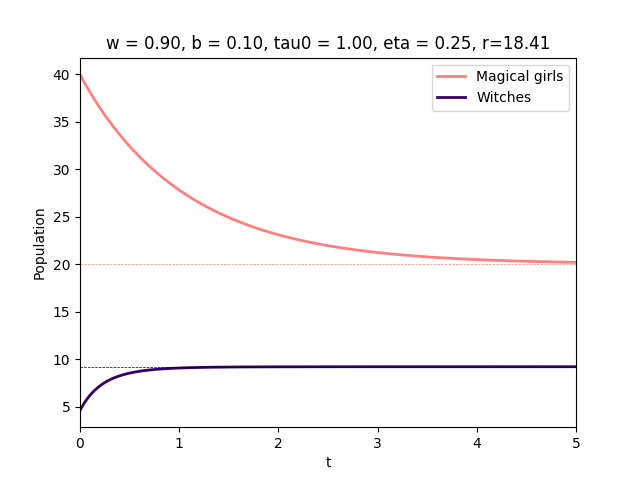
\includegraphics[width=0.7\textwidth]{fig1}
	\centering
	\caption{Model 1. Initial conditions: $M > M_{eq}$, $W < W_{eq}$.}	
	\label{fig1}
\end{figure}

\begin{figure}
	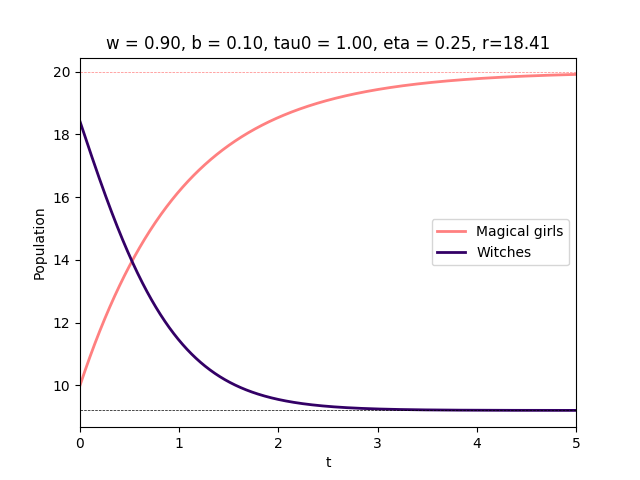
\includegraphics[width=0.7\textwidth]{fig2}
	\centering
	\caption{Model 2. Initial conditions: $M < M_{eq}$, $W > W_{eq}$.}	
	\label{fig2}
\end{figure}

\begin{figure}
	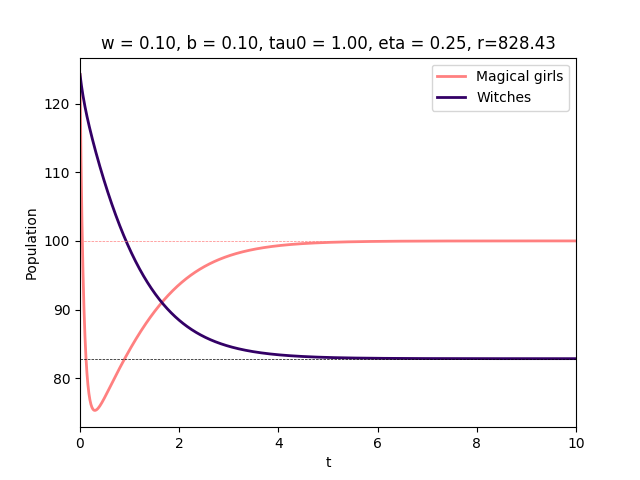
\includegraphics[width=0.7\textwidth]{fig3}
	\centering
	\caption{Model 3. Initial conditions: $M > M_{eq}$, $W > W_{eq}$. The low win rate ($w = 0.1)$ causes an oscillation in the magical girl population before equilibrium is reached.}	
	\label{fig3}
\end{figure}

Figures \ref{fig1}-\ref{fig3} show some possible scenarios. These start with off-equilibrium values of $M$ and $W$ and converge over time. The time scale is determined by setting $\tau_0=1$. As one can see, all the convergence is quick and without incident, regardless of starting conditions. Figure \ref{fig3} shows an example in which an oscillation of the magical girl population can be observed. This is the consequence of a specifically `soft' model, with a low win rate ($w=0.1$). While convergence eventually still occurs, this is another reason for why a high win rate for magical girls is generally desirable - as it tends to result in a faster and surer convergence of populations to their equilibrium values.

\section{Conclusions}
An idealised model describing the population dynamics of magical girls and witches in a closed environment has been developed and characterised. The model allows us some important and non trivial insights in the ecological balance of such populations, in particular:

\begin{itemize}
	\item that the density of witch population sustainable by a territory is independent of the population of magical girls, and only depends on the properties of the territory itself,
	\item that the population of magical girls is directly proportional to the recruitment rate, and
	\item that the energy production rate due to the decay of magical girls into witches is maximally efficient when the former have high rates of success in battle against the latter.
\end{itemize}

In practical field applications, of course, these considerations will need to be balanced with other requirements. For example, while a high recruitment rate and a perfect win rate would maximise energy production as per Eq. \ref{net_power}, they would actively work against the psychological needs of recruitment itself, which often relies on the threat posed by witches as a motivational factor. If witches are vastly outnumbered by magical girls and are dispatched quickly and reliably, the appeal of such arguments would be significantly weakened. Regardless, these results provide useful guidelines that need then to be integrated within the larger needs of ecological management.\newline
There are also potentially significant effects that have been ignored in this first model. Among them are any finite-size effects that could manifest in the situation in which an area was significantly overcrowded with witches or magical girls; the possibility, documented albeit of relatively small incidence, of internal combat and even murder within magical girls \cite{kyubey3}; and any effects due to the finiteness of the indigenous population if put under extreme stress due to either the drain of recruitment or the damage caused by witches. While some or all of these effects can matter in extreme circumstances, we believe that in the case of well-managed systems, the conditions for them to be important should never verify, and the results of this paper should hold. Nevertheless, the inclusion of such effects will be the object of study of future work.


\bibliographystyle{unsrt}
\bibliography{mweco}


\end{document}
